% results.tex — evaluation section. Numbers from:
%   bench_isal/results/DESKTOP-MDBVB0T-20261030-1146   (decode costs, i9-14900HX)
%   fecsim/results/20261030-1159                       (5,000 trials/point; 1,000 for 64-flow steps)
% Figures: copy fecsim/results/20261030-1159/figures/fig{1,3}*.png next to this file.

\section{Evaluation}
\label{sec:eval}

\subsection{Setup}

\paragraph{Decode cost.} We measure single-core median decode latency for 4\,KB packets on an
Intel Core i9-14900HX (AVX2, GFNI), Ubuntu~24.04 under WSL2, with Intel ISA-L~v2.31 and cm256
built from source. All decoders receive identical data, loss patterns and survivor sets, and every
decode is verified byte-for-byte. We compare three decoders:
\begin{itemize}
  \item ISA-L's documented decode path, which inverts the $k\times k$ survivor matrix for every loss pattern;
  \item cm256, which eliminates the received data and solves an $m'\times m'$ Cauchy system by LDU decomposition;
  \item erasure-count decoding~\cite{li2005patent} on ISA-L's GFNI kernel.
\end{itemize}

\paragraph{Network model.} A discrete-event simulator sends one RDMA message, or 64 messages in parallel
for a collective step, over a 100\,Gbps link with 4\,KB MTU. One-way delay is RTT/2 and losses are
Bernoulli. It compares:
\begin{itemize}
  \item go-back-N (GBN), as in commodity RoCE NICs;
  \item IRN-style selective repeat (SR)~\cite{irn};
  \item SR with a tail-loss probe after $2\times$RTT (SR+TLP);
  \item systematic RS($n,k$) FEC with a selective-repeat fallback.
\end{itemize}
FEC decode times are the measured medians above, queued on one core. The retransmission timeout is
100\,\textmu s for every scheme. For each point we report the best of the codes
RS(17,16), RS(18,16), RS(20,16), RS(34,32) and RS(36,32). The simulator reproduces 17 hand-derived
completion times exactly, and all schemes see the same random loss draws. We report the
99th-percentile completion time over 5{,}000 messages (1{,}000 collective steps).

\subsection{Decode cost}

ISA-L spends most of a cold decode on matrix inversion: 10--12\,\textmu s at $k{=}16$ and
56--60\,\textmu s at $k{=}32$, whereas its packet work takes only a few microseconds. Erasure-count
decoding on the same kernel removes almost all of the inversion cost. With one or two lost packets
and $k\ge16$ it decodes 11--43$\times$ faster than ISA-L, and 6--19\% slower than ISA-L with a
pre-cached decode matrix. Against cm256 it is 0.92--1.30$\times$ when one packet is lost
($k\ge16$) and 1.8--2.1$\times$ when two or more are lost. That gain comes from the GFNI kernel, not
the decoding algorithm, since both decoders solve the same $m'\times m'$ system.

\subsection{When does FEC beat retransmission?}

\begin{table}[t]
\centering
\caption{p99 completion of a collective step (slowest of 64 flows, 128\,KB each) at loss rate $10^{-3}$, in \textmu s.
``Best retransmission'' is the better of SR and SR+TLP.}
\label{tab:collective}
\begin{tabular}{rrrrrr}
\toprule
RTT (\textmu s) & Best retransmission & FEC, ISA-L & FEC, cm256 & FEC, erasure-count & FEC, free decode \\
\midrule
2  & 15.8 & 27.6 & 12.7 & 12.8 & 12.1 \\
5  & 23.3 & 29.1 & 14.2 & 14.3 & 13.6 \\
10 & 35.8 & 31.6 & 17.1 & 17.1 & 16.1 \\
25 & 73.3 & 39.5 & 24.6 & 24.6 & 23.6 \\
\bottomrule
\end{tabular}
\end{table}

\paragraph{Decode cost decides the winner.} Table~\ref{tab:collective} shows a 64-flow collective
step at $10^{-3}$ loss. With ISA-L's $k\times k$ decoder, FEC \emph{loses} to selective repeat with a
tail-loss probe at RTTs of 2 and 5\,\textmu s (27.6 vs.\ 15.8 and 29.1 vs.\ 23.3\,\textmu s). The
same FEC scheme with an erasure-count decoder \emph{wins} at every RTT, by 1.2--3.0$\times$, and
comes within 4--6\% of an FEC scheme with free decoding. Neither the code nor the loss process
changes between these runs, only the decoder. The same reversal appears across loss rates
(Figure~\ref{fig:collective}). At $10^{-4}$ loss and RTT 5\,\textmu s, erasure-count FEC takes
14.3\,\textmu s, retransmission 18.3\,\textmu s, and FEC with ISA-L 24.2\,\textmu s.

\paragraph{Why retransmission loses the tail.} A lost final packet produces no out-of-order arrival
to trigger a NAK, so plain SR and GBN wait for the timeout. Their p99 for a 64-flow step jumps from
18 to 118\,\textmu s between $10^{-4}$ and $10^{-3}$ loss. A tail-loss probe recovers most of this,
but not when the probe or several final packets are lost. At $10^{-2}$ loss SR+TLP again reaches
118\,\textmu s, while erasure-count FEC stays at 16.8\,\textmu s.

\paragraph{When FEC does not pay.} Parity costs bandwidth: 6.25\% for RS(17,16) and RS(34,32).
Below about $10^{-4}$ loss, or for single messages of 2\,MB and up, this overhead outweighs the
recovery benefit. For example, a single 2\,MB message at $10^{-3}$ loss and RTT 5\,\textmu s
completes in 173\,\textmu s with SR and in 181\,\textmu s with FEC. Figure~\ref{fig:ratio} maps the
boundary. FEC with an erasure-count decoder wins for small messages at loss rates of $10^{-3}$ and
above, and the region where it wins grows with RTT. ISA-L decoding shrinks that region to almost
nothing at RTTs of 5\,\textmu s or less.

\paragraph{Which erasure-count decoder matters little.} cm256 and erasure-count decoding on ISA-L's
kernel differ by at most 3.7\,\textmu s at the 99th percentile in every configuration we tested. Once decoding costs about
1\,\textmu s, RTT and serialisation dominate. The decisive difference is $k\times k$ inversion versus
erasure-count decoding, not which erasure-count implementation is used.

\begin{figure}[t]
\centering
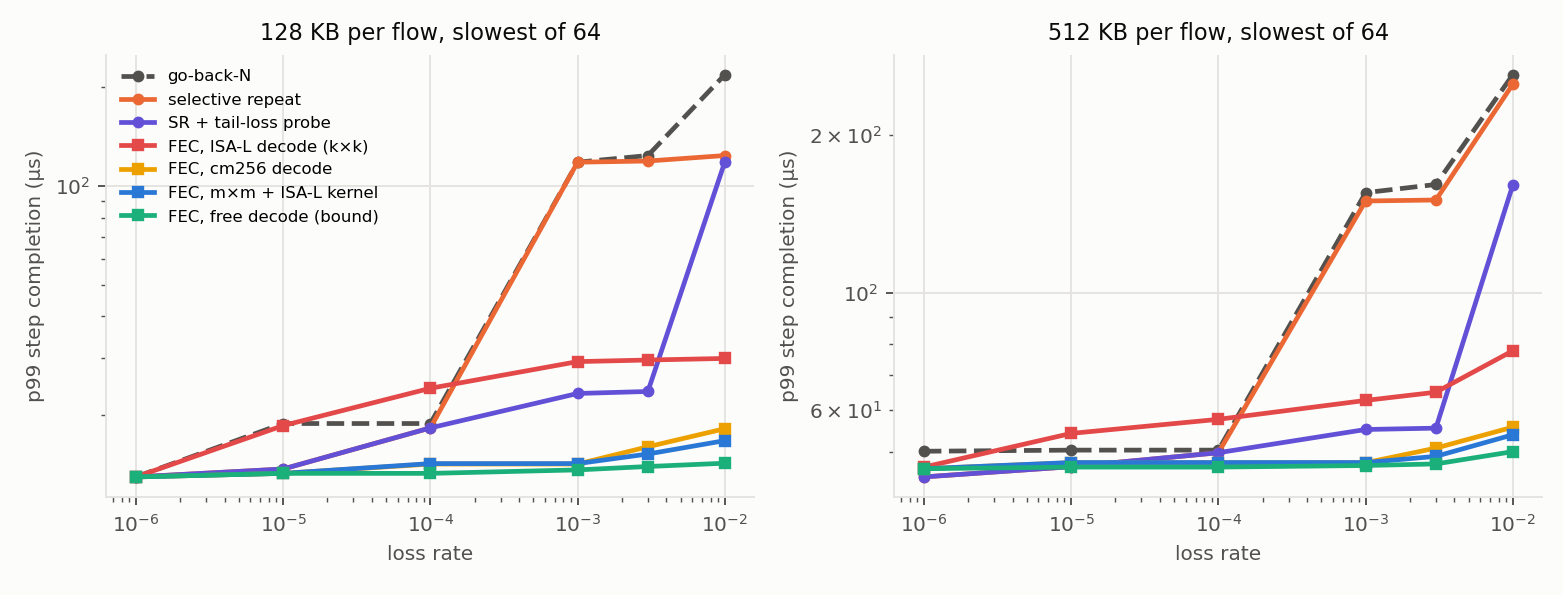
\includegraphics[width=\linewidth]{fig3_collective.png}
\caption{p99 completion of a 64-flow collective step versus loss rate (RTT 5\,\textmu s, 100\,Gbps).}
\label{fig:collective}
\end{figure}

\begin{figure*}[t]
\centering
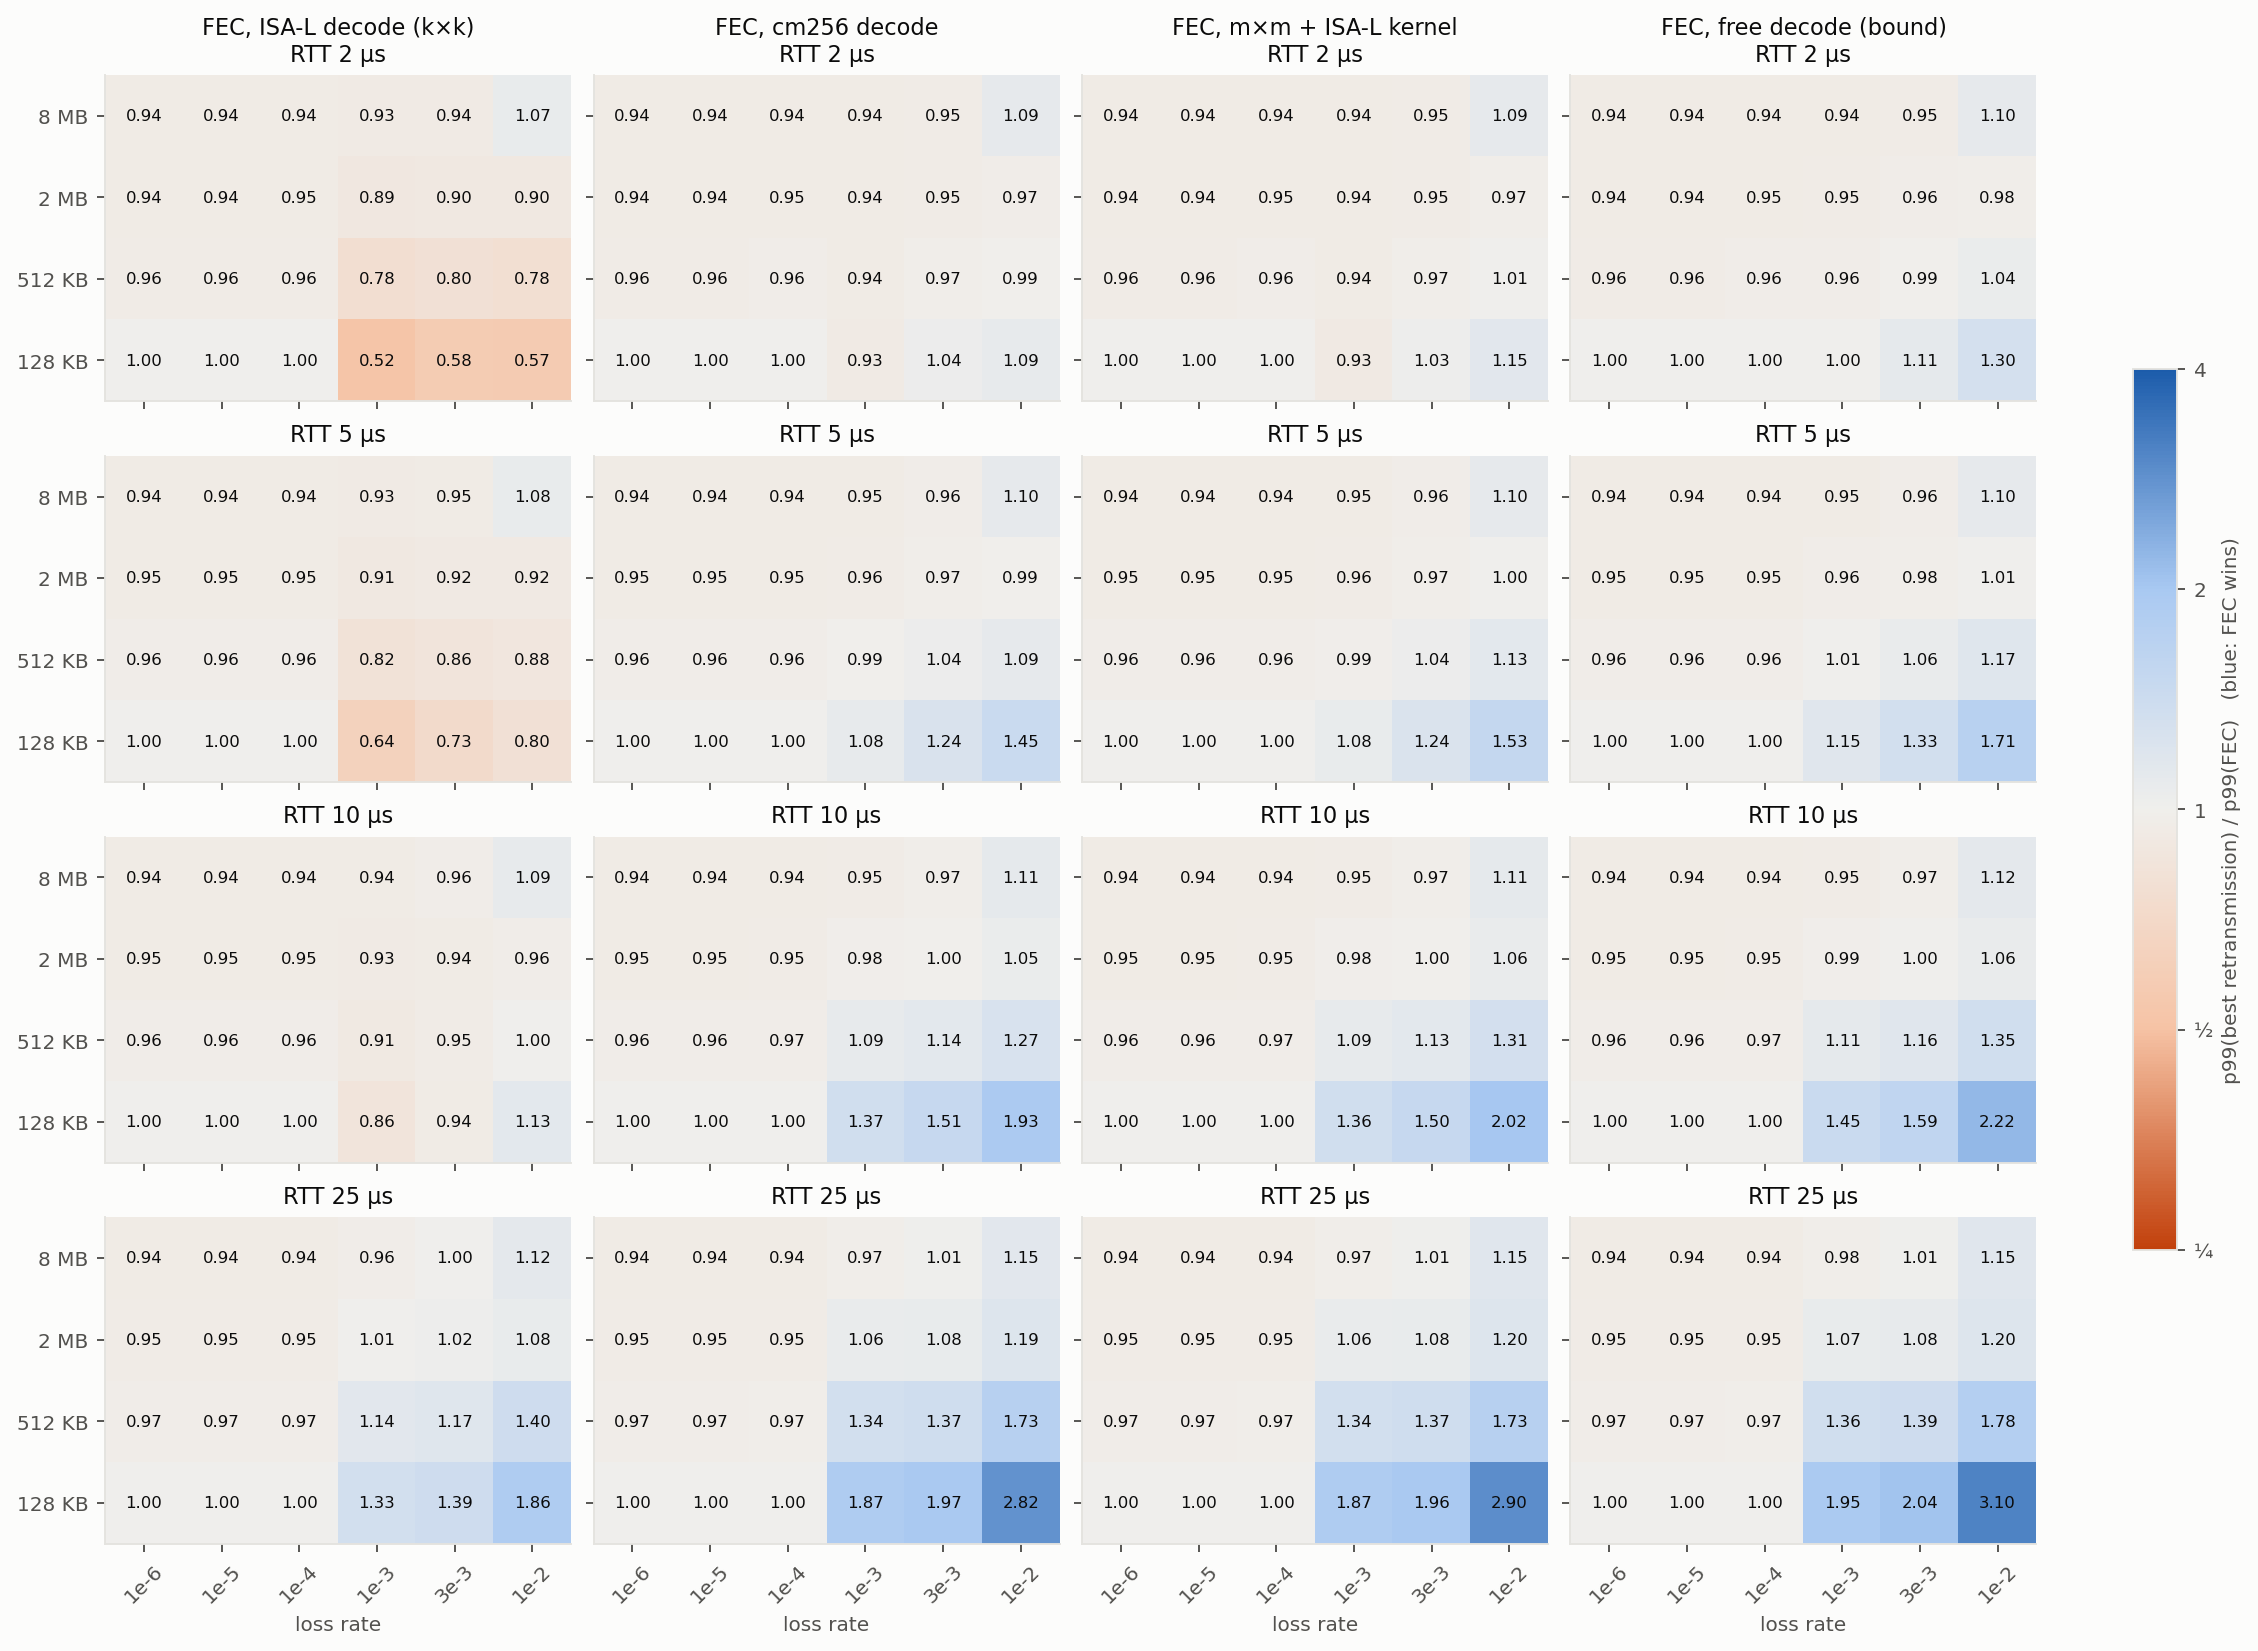
\includegraphics[width=\linewidth]{fig1_ratio_bernoulli.png}
\caption{p99(best retransmission)\,/\,p99(best FEC code) for a single flow, over loss rate and message
size. Rows are RTTs and columns are decoders. Blue means FEC wins.}
\label{fig:ratio}
\end{figure*}

\subsection{Limitations}
Our model has no congestion control, PFC or NIC pipeline. The flows in a collective step are
independent and do not share a bottleneck, the sender is not window-limited, and acknowledgements
are never lost. Decode costs come from one laptop CPU under WSL2. Losses are i.i.d.; our bursty
three-state model is not yet fitted to measured traces. Commodity RoCE timeouts are often far above
100\,\textmu s, which would favour FEC and SR+TLP further.
